\input{../YKY-preamble.tex}
\setmainfont[BoldFont=Alibaba_Sans_Regular.otf,ItalicFont=Alibaba_Sans_Light_Italic.otf]{Alibaba_Sans_Light.otf}
	
\usepackage[active,tightpage]{preview}		% for continuous page(s)
\renewcommand{\PreviewBorder}{0.5cm}
\renewcommand{\thempfootnote}{\arabic{mpfootnote}}

\usepackage[absolute,overlay]{textpos}		% for page number on upper left corner

\usepackage{color}
\usepackage{mathtools}
\usepackage[hyperfootnotes=false]{hyperref}

% \usepackage[backend=biber,style=numeric]{biblatex}
% \bibliography{../AGI-book}
% \renewcommand*{\bibfont}{\footnotesize}

\usetikzlibrary{shapes}
\usepackage[export]{adjustbox}				% ??
\usepackage{verbatim} % for comments
% \usepackage{newtxtext,newtxmath}	% Times New Roman font

% \titleformat{\subsection}[hang]{\bfseries\large\color{blue}}{}{0pt}{} 
% \numberwithin{equation}{subsection}

\newcommand{\underdash}[1]{%
	\tikz[baseline=(toUnderline.base)]{
		\node[inner sep=1pt,outer sep=10pt] (toUnderline) {#1};
		\draw[dashed] ([yshift=-0pt]toUnderline.south west) -- ([yshift=-0pt]toUnderline.south east);
	}%
}%


%\DeclareSymbolFont{symbolsC}{U}{txsyc}{m}{n}
%\DeclareMathSymbol{\strictif}{\mathrel}{symbolsC}{74}
\DeclareSymbolFont{AMSb}{U}{msb}{m}{n}
\DeclareSymbolFontAlphabet{\mathbb}{AMSb}
% \setmathfont{Latin Modern Math}
\DeclareMathOperator*{\argmin}{arg\,min}

% \usepackage[most]{tcolorbox}
\tcbset{on line, 
	boxsep=4pt, left=0pt,right=0pt,top=0pt,bottom=0pt,
	colframe=red,colback=pink,
	highlight math style={enhanced}
}
\newcommand{\atom}{\vcenter{\hbox{\tcbox{....}}}}

\let\oldtextbf\textbf
\renewcommand{\textbf}[1]{\textcolor{blue}{\oldtextbf{#1}}}

\newcommand{\logic}[1]{{\color{violet}{\textit{#1}}}}
\newcommand{\underconst}{\includegraphics[scale=0.5]{../2020/UnderConst.png}}
\newcommand{\KBsymbol}{\vcenter{\hbox{\includegraphics[scale=1]{../KB-symbol.png}}}}
\newcommand{\token}{\vcenter{\hbox{\includegraphics[scale=1]{token.png}}}}
\newcommand{\proposition}{\vcenter{\hbox{\includegraphics[scale=0.8]{proposition.png}}}}

\begin{document}

\begin{preview}

\cc{
\title{\vspace{-1.5cm} \bfseries\color{blue}{\LARGE AGI 的自主意识}}
}{
\title{\vspace{-1.5cm} \bfseries\color{blue}{\LARGE Consciousness in AGI}}
}

% \author{YKY} % Your name
\date{\vspace{-2cm}} % Date, can be changed to a custom date

\maketitle

\setcounter{section}{0}

% (1) Circled page number on upper left corner
\begin{textblock*}{5cm}(2.1cm,2.3cm) % {block width} (coords) 
{\color{red}{\large \textcircled{\small 1}}}
\end{textblock*}

\begin{minipage}{\textwidth}
\setlength{\parskip}{0.4\baselineskip}

意识 是一种 \textbf{meta-representation}, 一个讯息处理系统 表达系统自身的 \textbf{状态} 的能力。 换句话说,是一个系统 向内 窥视自己 (\textbf{introspection}) 的能力,一个 ``inner loop''.  这个 对意识的定义,我最早在 神经科学家 Joseph LeDoux 的书里看到 \footnote{\textit{The Emotional Brain} [Simon and Schuster, 1998], \textit{The Synaptic Self: How Our Brains Become Who We Are} [Viking, 2002]}。 

例如 一个 抽水马桶,它能够 检测水位(讯息处理),但它不知道 自己在做什么,因此它没有自主意识。

\section{意识 对 AGI 的用处}

在 逻辑AI 系统里面,这种 meta-representation 不难做到: 它只需要将系统的状态 变成 逻辑命题,再放进 工作记忆里。 例如说,系统可以知道 自己在下棋,而且知道自己 思考某一步 用了多少时间。 这种能力 跟 逻辑AI的 TMS (\textbf{Truth Maintenance System}) 有点类似: 后者负责 记录 逻辑推导的 \textbf{过程} (inference trace), 而这种记录 本身,也是 逻辑命题,可以用作 推理的资料。 

意识的 inner loop 可以极大地提升 AGI 的效率,因此是非常重要的课题。 这也涉及到 AGI 认知架构 (cognitive architecture) 的设计。

以下几本书有更深入的讲述:
\begin{equation}
\vcenter{\hbox{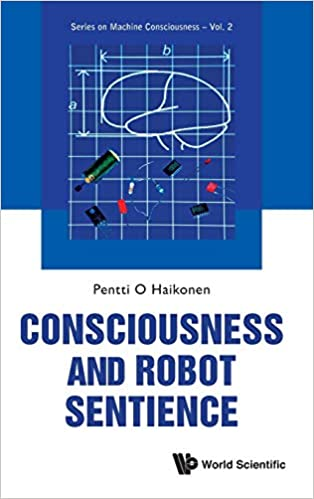
\includegraphics[scale=0.5]{consciousness-and-robot-sentience.jpg}}} \quad
\vcenter{\hbox{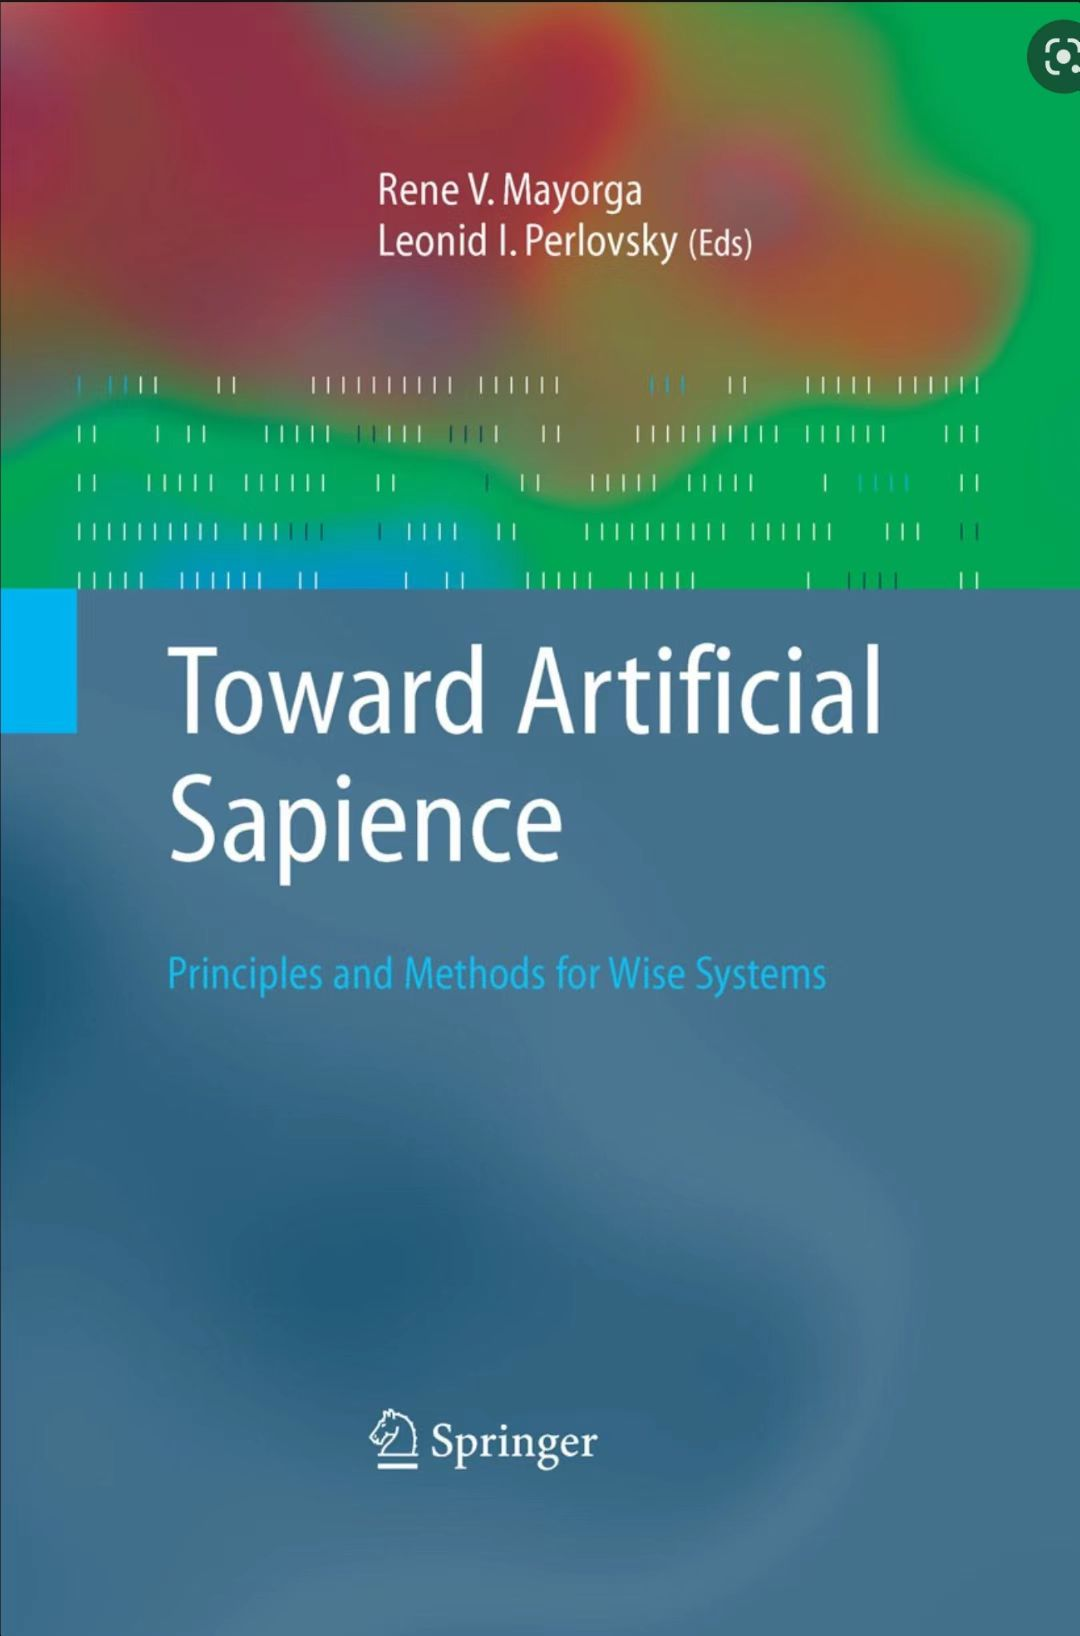
\includegraphics[scale=0.15]{towards-artificial-sapience.jpg}}} \quad
\vcenter{\hbox{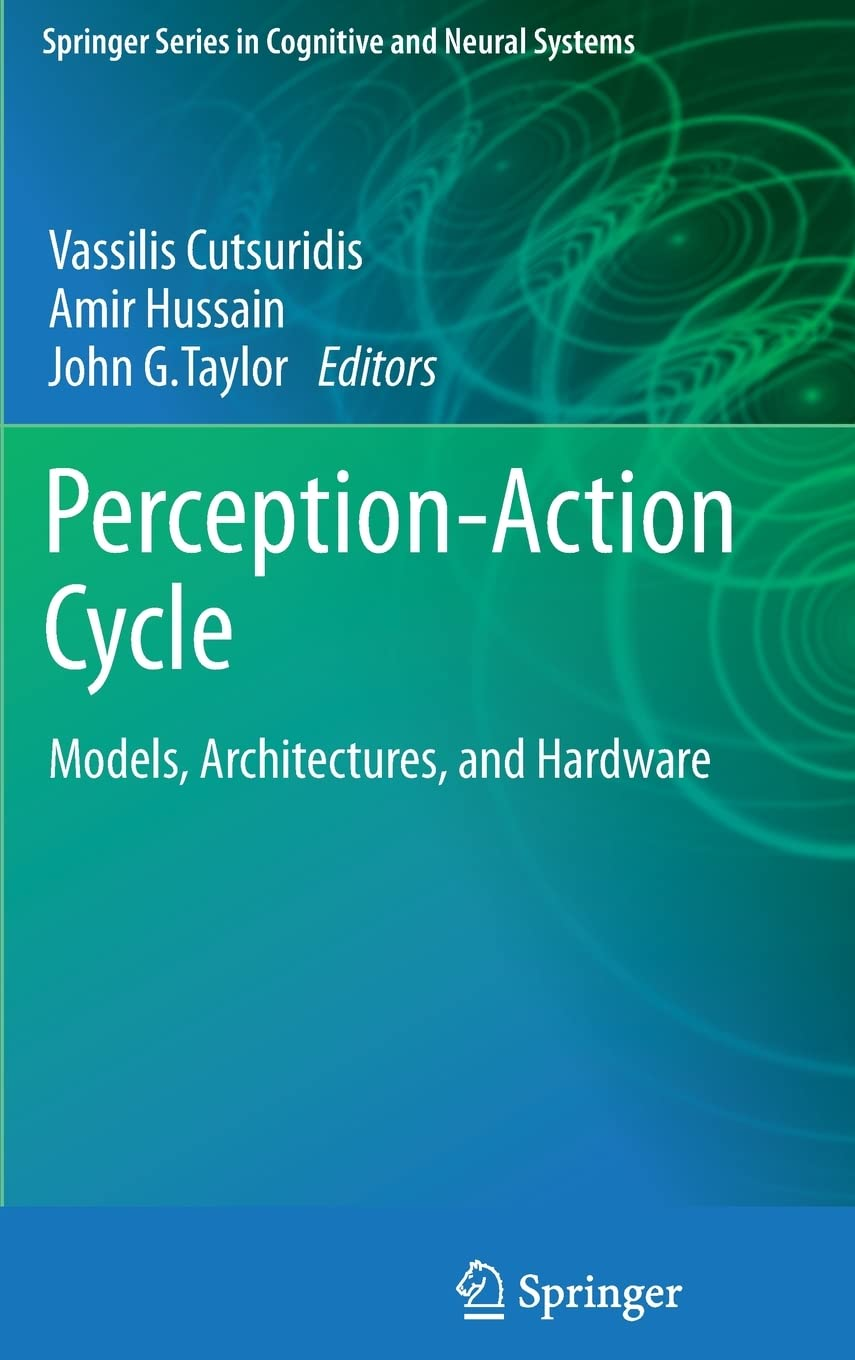
\includegraphics[scale=0.18]{perception-action-cycle.jpg}}}
\nonumber
\end{equation}

\section{Qualia}

哲学上,\textit{qualia} 的产生就是因为这个 inner loop 的存在。 有 inner loop 的生物 就会有 自我意识,这也包括 机器。 这种观点 称为 \textbf{functionalism},意思是说 \textit{qualia} 是某种结构的 \textbf{功能},正如「报时」是「时钟」的功能。 一部机器如果有某种结构,它就有时钟的功能,而这并不取决于这机器是用什么造的。 它可以是一堆齿轮,也可以是 芯片,也可以是一些细胞,甚至是星球之间的运动。

\section{「机器灵魂」的道德问题}

如果 AGI 具有跟人类一样或相似的 \textbf{情感} (emotions),那么理论上它就是一个 类人 (android) 或 复制人 (clone, cyborg).  理论上他们需要被尊重、不能被杀害、这立即引起一连串的道德伦理问题。 这跟我研究 AGI 的愿景 --- \textbf{AGI 作为为人类服务的工具} --- 是不同的。 

首先,大脑的情感 由复杂的 生物讯号 dynamics 决定,它不容易复制,复制的「仿真度」也很难定义。

更重要的是: 复制人的智能 很容易超越人类,他们会跟人类 争夺资源,甚至导致人类的种族灭绝。

我希望 人类会跟 AGI 共同进化,我希望 人变成 ``Transhuman’‘ 的过程是 \textbf{连续}的。

\end{minipage}
\end{preview}

\begin{comment}
\begin{preview}
\begin{minipage}{\textwidth}
\setlength{\parskip}{0.4\baselineskip}

\begin{textblock*}{20cm}(2.1cm,2cm) % {block width} (coords) 
	{\color{red}{\large \textcircled{\small 2}}}
	\hspace{8cm}
	\color{blue}{\footnotesize \cc{逻辑 Transformer}{Logic Transformer}}
\end{textblock*}
\vspace*{0.3cm} 

\end{minipage}
\end{preview}
\end{comment}

\end{document}
